\documentclass{article}
\usepackage{tikz}
\usepackage{pgfplots}
\pgfplotsset{compat=1.18}

\begin{document}

\title{LaTeX and TikZ/PGF: Applications and Benefits}
\author{Your Name}
\date{\today}
\maketitle

\section{Introduction}
TikZ and PGF are powerful tools for creating high-quality graphics in LaTeX documents. They support various types of diagrams and visualizations, making them invaluable for academic, professional, and technical documents.

\section{Applications of TikZ/PGF}
TikZ/PGF is widely used in fields such as:
\begin{itemize}
    \item Academic publishing: For creating mathematical diagrams, plots, and scientific illustrations.
    \item Engineering: For flowcharts, circuit diagrams, and mechanical schematics.
    \item Business: For organizational charts, process diagrams, and data visualizations.
    \item Education: For teaching materials and interactive graphics.
\end{itemize}

\section{Basic Diagram: Simple Shapes}
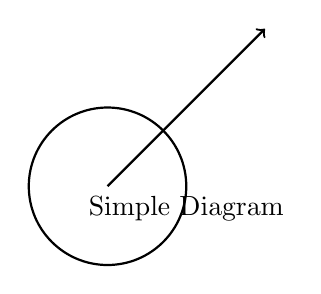
\begin{tikzpicture}
    \draw[thick] (0,0) circle (1cm);
    \draw[->, thick] (0,0) -- (2,2);
    \node[below] at (1,0) {Simple Diagram};
\end{tikzpicture}

\section{Graphs and Data Visualization}
TikZ/PGF excels in visualizing data. Below is an example of a bar chart:

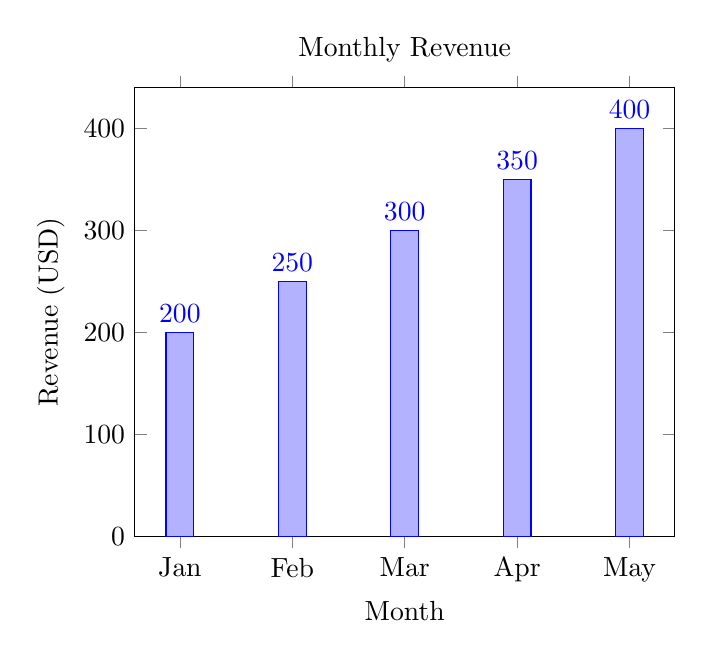
\begin{tikzpicture}
\begin{axis}[
    title={Monthly Revenue},
    xlabel={Month},
    ylabel={Revenue (USD)},
    symbolic x coords={Jan, Feb, Mar, Apr, May},
    xtick=data,
    ybar,
    ymin=0,
    bar width=10pt,
    nodes near coords
]
\addplot coordinates {(Jan,200) (Feb,250) (Mar,300) (Apr,350) (May,400)};
\end{axis}
\end{tikzpicture}

\section{Complex Network Diagrams}
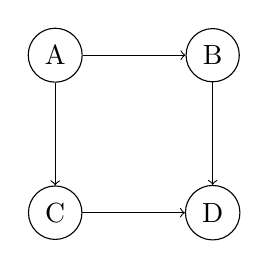
\begin{tikzpicture}[node distance=2cm]
    \node[draw, circle] (A) {A};
    \node[draw, circle, right of=A] (B) {B};
    \node[draw, circle, below of=A] (C) {C};
    \node[draw, circle, below of=B] (D) {D};
    \draw[->] (A) -- (B);
    \draw[->] (A) -- (C);
    \draw[->] (B) -- (D);
    \draw[->] (C) -- (D);
\end{tikzpicture}

\section{Flowcharts}
Flowcharts are essential in many fields, and TikZ/PGF simplifies their creation:
\begin{tikzpicture}[node distance=2cm, thick]
    \node[startstop] (start) {Start};
    \node[process, below of=start] (step1) {Step 1};
    \node[decision, below of=step1] (decision) {Decision?};
    \node[process, right of=decision, xshift=3cm] (step2) {Step 2};
    \node[startstop, below of=decision] (end) {End};
    \draw[->] (start) -- (step1);
    \draw[->] (step1) -- (decision);
    \draw[->] (decision) -- node[midway, above] {Yes} (step2);
    \draw[->] (decision) -- node[midway, left] {No} (end);
    \draw[->] (step2) |- (step1);
\end{tikzpicture}

\section{Geometric Figures}
TikZ/PGF is excellent for creating geometric illustrations:
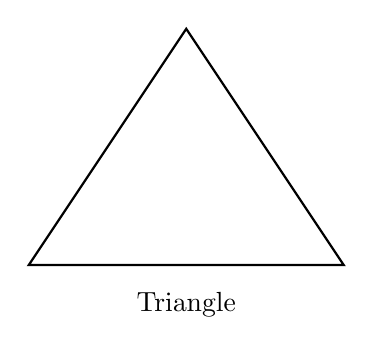
\begin{tikzpicture}
    \draw[thick] (0,0) -- (4,0) -- (2,3) -- cycle;
    \node at (2,-0.5) {Triangle};
\end{tikzpicture}

\section{Tables with PGFPlots}
PGFPlots allows for creating dynamic tables with visual enhancements:

\pgfplotstabletypeset[
    col sep=comma,
    string type,
    every head row/.style={
        before row=\hline,after row=\hline},
    every last row/.style={after row=\hline},
]{
Field, 2010, 2020
Mathematics, 50, 80
Engineering, 70, 120
Business, 40, 70
Education, 60, 100
}

\section{Advanced 3D Graphics}
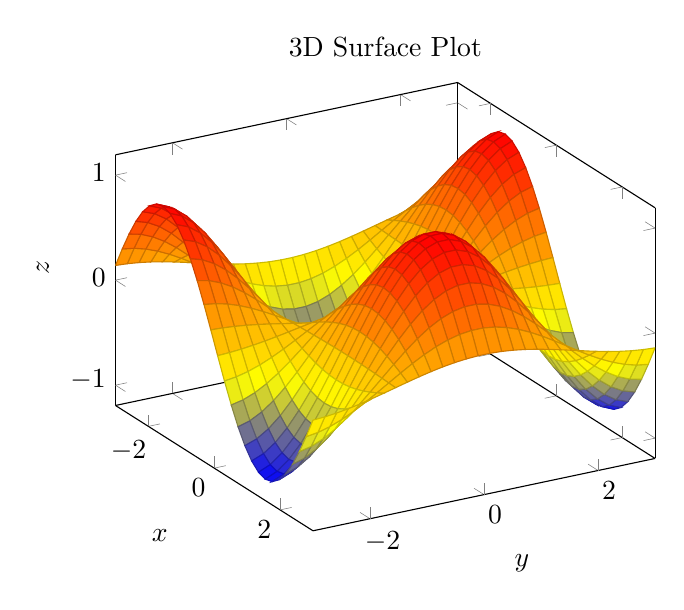
\begin{tikzpicture}
\begin{axis}[
    view={60}{30},
    title={3D Surface Plot},
    xlabel={$x$},
    ylabel={$y$},
    zlabel={$z$},
    domain=-3:3,
    y domain=-3:3,
    samples=30,
]
\addplot3[surf] {sin(deg(x)) * cos(deg(y))};
\end{axis}
\end{tikzpicture}

\section{Enhancing Work with TikZ/PGF}
Using TikZ/PGF offers several advantages:
\begin{itemize}
    \item Consistent styling across all graphics.
    \item Integration with LaTeX for high-quality typesetting.
    \item Scalability without loss of quality.
    \item Automation and reusability of elements for complex projects.
\end{itemize}

\section{Applications by Profession}

\subsection{Academia and Education}
LaTeX is extensively used in academia for creating professional-grade documents, lecture notes, and books. TikZ/PGF enhances these documents with clear and customizable diagrams, aiding in teaching complex concepts.

\subsubsection*{Example: Venn Diagram}
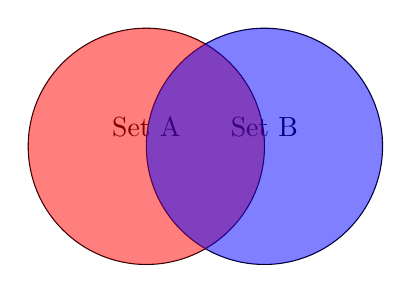
\begin{tikzpicture}
\draw (0,0) circle [radius=1.5] node [above] {Set A};
\draw (1.5,0) circle [radius=1.5] node [above] {Set B};
\fill[red,opacity=0.5] (0,0) circle [radius=1.5];
\fill[blue,opacity=0.5] (1.5,0) circle [radius=1.5];
\end{tikzpicture}

\subsubsection*{Benefits}
\begin{itemize}
    \item Simplifies creation of structured documents.
    \item Produces high-quality, consistent outputs.
\end{itemize}

\subsection{Scientific Research}
In scientific research, LaTeX is a go-to tool for writing papers, theses, and reports. TikZ/PGF enables precise visualization of experimental data and mathematical models.

\subsubsection*{Example: Graph of Experimental Data}
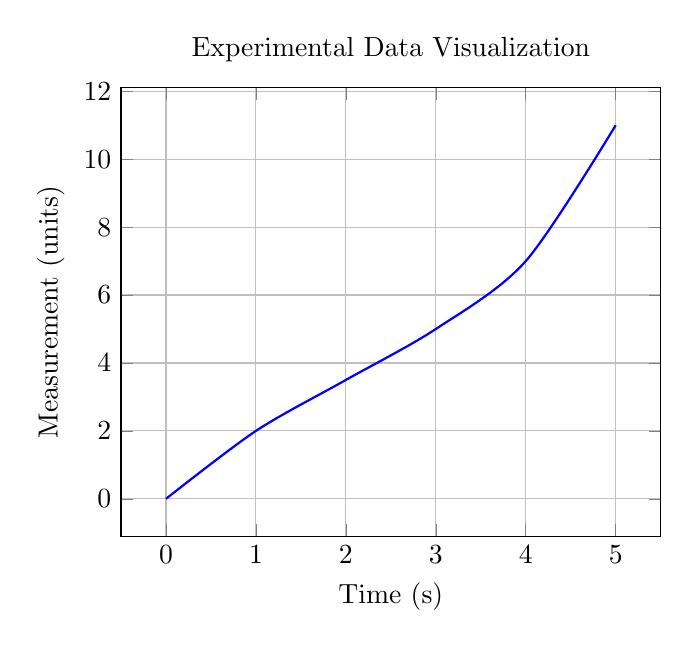
\begin{tikzpicture}
\begin{axis}[
    title={Experimental Data Visualization},
    xlabel={Time (s)},
    ylabel={Measurement (units)},
    grid=major
]
\addplot[smooth,blue,thick] coordinates {
    (0,0) (1,2) (2,3.5) (3,5) (4,7) (5,11)};
\end{axis}
\end{tikzpicture}

\subsubsection*{Benefits}
\begin{itemize}
    \item High-quality illustrations for journals.
    \item Flexible formatting for mathematical equations.
\end{itemize}

\subsection{Engineering}
Engineers leverage LaTeX and TikZ for technical drawings, circuit diagrams, and process visualizations.

\subsubsection*{Example: Circuit Diagram}
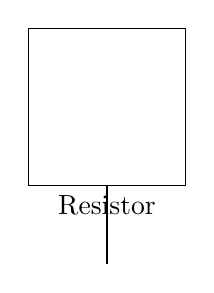
\begin{tikzpicture}
\draw (0,0) -- (2,0) node[midway,below] {Resistor} -- (2,2) -- (0,2) -- cycle;
\draw (1,0) -- (1,-1);
\end{tikzpicture}

\subsubsection*{Benefits}
\begin{itemize}
    \item Precise technical schematics.
    \item Customizable components for clarity.
\end{itemize}

\subsection{Mining}
In mining, LaTeX and TikZ are used for geological diagrams, data visualization, and technical documentation.

\subsubsection*{Example: Geological Layer Diagram}

\begin{tikzpicture}
\fill[gray] (0,0) rectangle (4,1) node[midway]{Layer 1};
\fill[brown] (0,1) rectangle (4,2) node[midway]{Layer 2};
\fill[green] (0,2) rectangle (4,3) node[midway]{Layer 3};
\end{tikzpicture}

\subsubsection*{Benefits}
\begin{itemize}
    \item Custom geological diagrams.
    \item Clear and accurate data representation.
\end{itemize}

\subsection{Software Development}
LaTeX is ideal for documenting code and creating visual representations of algorithms. TikZ/PGF aids in UML diagrams and flowcharts.

\subsubsection*{Example: UML Diagram}
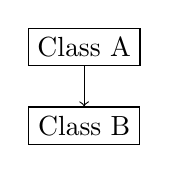
\begin{tikzpicture}
\node[draw] (A) {Class A};
\node[draw,below of=A] (B) {Class B};
\draw[->] (A) -- (B);
\end{tikzpicture}

\subsubsection*{Benefits}
\begin{itemize}
    \item Professional software documentation.
    \item Easy sharing of complex ideas visually.
\end{itemize}

\subsection{Physics}
Physicists use LaTeX for papers, and TikZ for detailed physics illustrations, such as forces and vectors.

\subsubsection*{Example: Force Diagram}
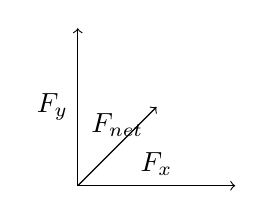
\begin{tikzpicture}
\draw[->] (0,0) -- (2,0) node[midway,above] {$F_x$};
\draw[->] (0,0) -- (0,2) node[midway,left] {$F_y$};
\draw[->] (0,0) -- (1,1) node[midway,above] {$F_{net}$};
\end{tikzpicture}

\subsubsection*{Benefits}
\begin{itemize}
    \item Precise physics visualizations.
    \item Clear representation of forces and concepts.
\end{itemize}

\subsection{Aeronautics}
Aeronautical engineers use LaTeX for technical documentation and TikZ for visualizing aerodynamic models.

\subsubsection*{Example: Airflow Visualization}
\begin{tikzpicture}
\draw[blue,->] (0,1) -- (5,1);
\draw[blue,->] (0,2) .. controls (2,3) .. (5,2);
\end{tikzpicture}

\subsubsection*{Benefits}
\begin{itemize}
    \item Precise airflow models.
    \item Custom illustrations for technical analysis.
\end{itemize}

\subsection{Big Data}
Big data analysts use LaTeX and TikZ for documenting analytical processes and visualizing data trends.

\subsubsection*{Example: Data Flow Chart}
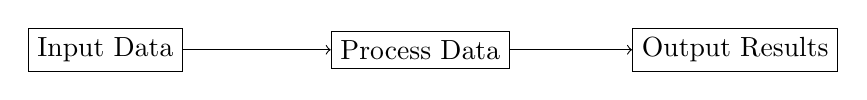
\begin{tikzpicture}
\node[draw] (Input) {Input Data};
\node[draw,right of=Input,xshift=3cm] (Process) {Process Data};
\node[draw,right of=Process,xshift=3cm] (Output) {Output Results};
\draw[->] (Input) -- (Process);
\draw[->] (Process) -- (Output);
\end{tikzpicture}

\subsubsection*{Benefits}
\begin{itemize}
    \item Clear representation of processes.
    \item Effective communication of data insights.
\end{itemize}

\subsection{Machine Learning}
In machine learning, LaTeX and TikZ are used for academic papers, algorithm visualizations, and model representation.

\subsubsection*{Example: Neural Network Diagram}
\begin{tikzpicture}
\foreach \i in {1,...,3} {
    \node[circle,draw] (I\i) at (0,-\i) {};
    \node[circle,draw] (H\i) at (2,-\i) {};
    \node[circle,draw] (O\i) at (4,-\i) {};
    \foreach \j in {1,...,3} {
        \draw[->] (I\i) -- (H\j);
        \draw[->] (H\i) -- (O\j);
    }
}
\end{tikzpicture}

\section{Conclusion}
TikZ/PGF transforms LaTeX documents by adding high-quality, customizable graphics, enhancing readability and professionalism. Mastery of these tools empowers users to create impactful visuals tailored to diverse applications.

\end{document}
